% =====================================================================
%  Coverage-Guided Property-Based Testing — Master Thesis
%  Mihnea-Andrei Blotiu, UNSTPB / Faculty of Automatic Control and Computers
%
%  Self-contained LaTeX (report class). The chapter bodies are written to be
%  pasted directly into the official UPB diploma template; if compiled stand-
%  alone, `pdflatex thesis.tex` twice resolves the references. Figures are the
%  ones generated by the project under ../images and the analysis charts under
%  ../../engine/reports/statistics/_summary (regenerate with `make full`).
% =====================================================================
\documentclass[11pt,a4paper]{report}

\usepackage[utf8]{inputenc}
\usepackage[T1]{fontenc}
\usepackage[a4paper,margin=2.5cm]{geometry}
\usepackage{amsmath,amssymb}
\usepackage{graphicx}
\usepackage{booktabs}
\usepackage{xcolor}
\usepackage{listings}
\usepackage{caption}
\usepackage{enumitem}
\usepackage[hidelinks]{hyperref}

\definecolor{kw}{RGB}{47,92,138}
\definecolor{cmt}{RGB}{120,120,120}
\definecolor{str}{RGB}{31,138,112}
% Listings are used only for language-agnostic PSEUDOCODE (no real Scala),
% so the keyword set is the pseudocode vocabulary, not a language's.
\lstset{
  basicstyle=\ttfamily\footnotesize,
  keywordstyle=\color{kw}\bfseries,
  commentstyle=\color{cmt}\itshape,
  numbers=left, numberstyle=\tiny\color{cmt}, stepnumber=1, numbersep=8pt,
  breaklines=true, frame=single, framesep=4pt, captionpos=b,
  showstringspaces=false, tabsize=2, columns=fullflexible,
  morekeywords={function,for,foreach,in,if,else,then,return,match,case,while,repeat,until,and,or,not,do,end,each,defined,empty,NONE}
}
\renewcommand{\lstlistingname}{Pseudocode}

\title{Coverage-Guided Property-Based Testing}
\author{Mihnea-Andrei Blotiu}
\date{2026}

\begin{document}

% --------------------------------------------------------------------
\begin{titlepage}
\centering
{\large NATIONAL UNIVERSITY OF SCIENCE AND TECHNOLOGY POLITEHNICA BUCHAREST\par}
{\large FACULTY OF AUTOMATIC CONTROL AND COMPUTERS\par}
{\large COMPUTER SCIENCE AND ENGINEERING DEPARTMENT\par}
\vfill
{\Huge\bfseries MASTER THESIS\par}
\vspace{1.5cm}
{\LARGE Coverage-Guided Property-Based Testing\par}
{\large A Composable Framework and Its Empirical Evaluation against Random Generation\par}
\vfill
\begin{flushright}
\textit{Author:} \quad Mihnea-Andrei Blotiu\\[0.4cm]
\textit{Thesis advisor:} \quad \c{S}.l. Dr. Ing. Mihnea-Cosmin Muraru
\end{flushright}
\vfill
{\large BUCHAREST, 2026\par}
\end{titlepage}

% --------------------------------------------------------------------
\chapter*{Abstract}
\addcontentsline{toc}{chapter}{Abstract}

\noindent\textbf{Abstract (EN).}
Property-based testing validates code by checking general properties on automatically generated
inputs. Its effectiveness depends entirely on the generator: a purely random generator treats the
system under test as a black box and rarely reaches branches guarded by exact literals, narrow
numeric targets, or highly structured inputs. This thesis asks to what extent, and at what cost,
\emph{coverage-guided} property-based testing improves over random generation. We design and implement a
Scala framework in which a strategy is a composition of independent, coverage-guided tactics over a
single, honest baseline that is literally stock ScalaCheck. Two tactics are studied: a constant
\emph{pool} mined from the source and a value-level \emph{mutation} engine over coverage-growing inputs.
The four strategies are exactly the subsets of these two tactics, enabling a clean ablation. The framework
is evaluated on a purpose-built benchmark of 27 methods across five categories, reporting both
method-local statement coverage and branch-marked statement coverage over repeated seeds. Each tactic owns a
distinct niche: the pool is intended for exact-literal gates, while mutation is intended for structured
inputs such as ordered lists and shaped trees.

\vspace{0.6cm}
\noindent\textbf{Sinopsis (RO).}
Testarea bazat\u{a} pe propriet\u{a}\c{t}i valideaz\u{a} codul verificând propriet\u{a}\c{t}i generale pe
intr\u{a}ri generate automat, iar eficacitatea ei depinde în întregime de generator: unul pur aleator
trateaz\u{a} sistemul ca o cutie neagr\u{a} \c{s}i atinge rar ramurile p\u{a}zite de literali exac\c{t}i, \c{t}inte
numerice înguste sau intr\u{a}ri puternic structurate. Lucrarea studiaz\u{a} în ce m\u{a}sur\u{a} \c{s}i cu ce
cost testarea ghidat\u{a} de acoperire dep\u{a}\c{s}e\c{s}te generarea aleatoare. Propunem un cadru în Scala în
care o strategie este o compunere de tactici independente, ghidate de acoperire, peste o baz\u{a} onest\u{a}
identic\u{a} cu ScalaCheck. Studiem dou\u{a} tactici: un \emph{pool} de constante întregi extrase din surs\u{a}
\c{s}i o \emph{muta\c{t}ie} la nivel de valoare. Evaluarea folose\c{s}te un benchmark de 27 de metode peste
cinci categorii \c{s}i raporteaz\u{a} atât acoperire de instruc\c{t}iuni, cât \c{s}i acoperire de instruc\c{t}iuni
marcate ca ramuri de scoverage. Fiecare tactic\u{a} are o ni\c{s}\u{a} distinct\u{a}.

\tableofcontents

% ====================================================================
\chapter{Introduction}
\label{ch:intro}

As software touches more and more areas of our daily lives, ensuring its correctness has become an
important ongoing research subject and a real challenge. We start by establishing the broader context of
the software-testing research area, looking at different ways in which software validation is approached
today. We then narrow down to one specific problem that we address while emphasising both the objectives
and the main research question of the paper. In the end, we present the proposed solution through a
high-level description and provide a short overview of our contributions and results, as well as a
description of the structure of the rest of the paper.

\section{Context and Motivation}
\label{sec:context}

Since the beginning of engineering, its role in human life has progressively expanded, shaping nearly
every aspect of modern society. An important part of innovation is represented by software systems, which
have become deeply embedded in applications ranging from simple tools to critical domains. The likelihood
of major issues — unintended behaviour, bugs, errors, or vulnerabilities — grows as these systems become
more complex; such undiscovered issues can lead to costly consequences or significant risks~\cite{nist2002}.

Widely adopted solutions for validating software include testing and formal verification, used as
practical means of increasing confidence that a system behaves as intended. Both Myers et al.~\cite{myers}
and Claessen and Hughes~\cite{claessen2000} report that roughly half of the time spent in software
development is invested in testing. Figure~\ref{fig:confidence} arranges several validation techniques
along an axis of increasing confidence from left to right.

\begin{figure}[t]
\centering
\fbox{\parbox{0.9\textwidth}{\centering\vspace{2mm}
\textsf{Manual testing} \quad$\longrightarrow$\quad \textsf{Property-based testing} \quad$\longrightarrow$\quad \textsf{Formal verification}\vspace{2mm}}}
\caption{Confidence in correctness, from sampled inputs to mathematical proof.}
\label{fig:confidence}
\end{figure}

At the leftmost end lies manual testing, a general term that includes unit, functional, integration, and
end-to-end testing. The programmer selects specific input values based on personal judgement, executes the
program, and checks the output against the expected result. While straightforward and widely used in
industry, the confidence it provides is limited by the developer's ability to anticipate meaningful
scenarios~\cite{garousi}. At the opposite end stands formal verification, where validation is done by
mathematical proof rather than by sampling: one can demonstrate that a property holds universally. This
offers the highest confidence, but the proof effort often exceeds the implementation effort, and formal
methods have not been widely adopted in industry ``except, arguably, in the development of critical
systems in certain domains''~\cite{woodcock}.

Between the two lies property-based testing (PBT), a family of methods that combines elements of both. As
in formal verification, the developer writes general properties the system should satisfy; but rather than
proving them, PBT attempts to falsify them by automatically generating a large number of inputs and
executing the program in search of counterexamples~\cite{claessen2000}. PBT variants differ in how inputs
are generated: the simplest draws them at random, while more sophisticated strategies use runtime metrics
to guide subsequent values. This thesis concerns one strategy from the latter category — \emph{coverage-guided}
property-based testing — which uses runtime coverage information to influence the next generated inputs. We
discuss the limitations of purely random generation, contrast them with coverage-guided generation,
develop a framework that puts the approach into practice, and compare the two in terms of code coverage on
a benchmark designed to highlight hard-to-reach branches.

\section{Problem}
\label{sec:problem}

To obtain meaningful coverage, property-based testing relies almost entirely on generators to provide the
input values fed to the system under test (SUT). A property can only be exercised by inputs that actually
reach the relevant branches, so the overall coverage of a function depends directly on the quality of the
generated inputs. Many PBT frameworks treat the SUT as a black box and generate inputs randomly and
independently of one another. This is simple, popular, and often effective for shallow behaviour, but it
struggles with deep program paths and with highly constrained or structured inputs. As Hamlet~\cite{hamlet}
observes, random testing does not target any particular part of the program; whether more or fewer paths
are executed depends entirely on chance.

The fundamental issue is that no information about the code under test is taken into account, which can
lead to poor results and significant wasted effort beyond a certain point. Even if intuition suggests that
feeding runtime information back into the generators should help, the actual benefits are not immediately
evident. Identifying the conditions under which this idea brings advantages, and measuring how substantial
or negligible the benefits are in different cases, are among the main subjects studied in this thesis.

\section{Research Questions}
\label{sec:rq}

This thesis explores how a coverage-guided property-based testing framework compares to one that uses a
purely random generation strategy. The two focus areas are how much coverage each strategy can ultimately
achieve and how efficiently it gets there, measured by the number of inputs required. The study is guided
by one main research question:

\begin{quote}\itshape
\textbf{Main Question.} To what extent and at what cost does coverage-guided property-based testing improve
over a purely random strategy, both in terms of the code coverage ultimately achieved and the number of
inputs required to reach it?
\end{quote}

To answer it, we explore the following auxiliary questions:
\begin{enumerate}[label=RQ\arabic*., leftmargin=2.2cm]
  \item What are the limitations of purely random input generation in PBT frameworks, and in which kinds of tested code are those limitations emphasised?
  \item How can runtime coverage information from the SUT be collected during execution, and how can it be fed back to the input generators?
  \item How can coverage information be used by different generation strategies to create inputs that are effective at exploring new branches?
  \item On what classes of programs does the coverage-guided approach yield the largest improvements over the random baseline, considering both coverage and the number of inputs required?
  \item What overhead does a coverage-guided framework introduce, and under what circumstances is the effort outweighed by the benefits?
\end{enumerate}

\section{Objectives}
\label{sec:objectives}

The objectives of the project follow directly from the research questions:
\begin{enumerate}[leftmargin=1.6em]
  \item Build a framework in which random generation is an \emph{honest} baseline — identical to a standard PBT tool — so any measured difference is attributable to guidance and not to an unfair re-implementation.
  \item Collect branch-coverage feedback from the SUT at runtime, after every input, and expose it to the generators (RQ2).
  \item Design several coverage-guided generation strategies that exploit this feedback in different ways, and a uniform abstraction under which they compose (RQ3).
  \item Construct a benchmark that isolates the kinds of branches each strategy is meant to address, and quantify — with appropriate statistics — when guidance helps and by how much (RQ1, RQ4).
  \item Measure the runtime overhead the guidance introduces, to judge when it is worthwhile (RQ5).
\end{enumerate}

\section{Proposed Solution}
\label{sec:proposed-intro}

We propose a Scala framework in which a \emph{strategy} reads live coverage feedback and chooses the next
typed generator. The random strategy is plain random generation and is implemented as literally stock
ScalaCheck, so the baseline is beyond suspicion. Two guided sources are studied: a constant \emph{pool} that
draws from literals mined from the source code, and a value-level \emph{mutation} engine that perturbs inputs
which previously grew coverage. The four strategies we evaluate are exactly the combinations of these two
sources, which turns the comparison into a clean ablation study.

\section{Obtained Results}
\label{sec:results-intro}

On a benchmark of 27 methods across five categories, evaluated over repeated seeds, the framework compares
the random baseline with the pool, mutation, and composed pool-mutation strategies. The analysis reports
both method-local statement coverage and branch-marked statement coverage, together with time-to-coverage
curves, throughput, Vargha--Delaney effect sizes, and Mann--Whitney significance tests. Each tactic owns a
distinct niche — the pool cracks exact-literal gates, and mutation cracks incrementally-built structured
inputs — while the numeric-search category records cases that the current tactics are not expected to solve.

\section{Contributions}
\label{sec:contributions}

\begin{enumerate}[leftmargin=1.6em]
  \item \textbf{A scoverage-backed feedback loop} that maps runtime hits to method-local source targets and reports both statement and branch-marked statement coverage.
  \item A unifying \emph{tactic} abstraction that expresses literal pooling and value-level mutation as interchangeable, coverage-guided components over one generator type class, with the random baseline preserved exactly as stock ScalaCheck (Chapter~\ref{ch:solution}).
  \item A purpose-built benchmark organised as a progression of niches, and a repeated-seed evaluation pipeline reporting effect size ($\hat{A}_{12}$) and significance (Mann--Whitney $U$) per the Arcuri--Briand protocol~\cite{arcuri2014} (Chapter~\ref{ch:eval}).
  \item An empirical characterisation of \emph{when} each mechanism helps: literal pooling targets exact constants, mutation targets structured inputs, and numeric-search examples expose what remains hard without a numeric-distance tactic.
\end{enumerate}

\section{Structure}
\label{sec:structure}

The rest of the paper is structured as follows. Chapter~\ref{ch:background} introduces the technical
concepts and necessary background. Chapter~\ref{ch:related} positions the paper in the broader research
landscape. Chapter~\ref{ch:solution} introduces the high-level proposed solution and the design ideas
behind it, while Chapter~\ref{ch:impl} delves into the technologies used and the low-level implementation.
Chapter~\ref{ch:eval} introduces the evaluation benchmark and discusses the obtained results.
Chapter~\ref{ch:conclusions} concludes by presenting general findings, limitations, and future work.

% ====================================================================
\chapter{Background}
\label{ch:background}

This chapter presents the concepts required to understand the ideas behind coverage-guided property-based
testing. We introduce the vocabulary of software testing, narrow down to property-based testing and its
central concepts — properties and generators — then present code coverage as a measure of how thoroughly a
test exercises a program, and finally the two ideas that guidance borrows from neighbouring fields: search-based
testing with a branch-distance metric, and mutation-based, coverage-guided fuzzing.

\section{Software Testing}
\label{sec:testing}

When developing a software system, writing functional code is only one step of the process; testing comes
immediately after. Myers et al.~\cite{myers} describe testing as ``the process of executing a program with
the intent of finding errors''. Testing methods are classified by several criteria. By the amount of code
exercised, we distinguish unit testing (isolating a single behaviour), integration testing (combining
several components), and end-to-end testing (validating system specifications). Orthogonally, by the
knowledge of the implementation, we distinguish \emph{black-box} testing, which considers only the
specification, from \emph{white-box} (or structural) testing, which uses knowledge of the code's internal
structure. The distinction is central to this thesis: a purely random generator is black-box, whereas a
coverage-guided generator is grey-box — it does not read the source semantics but does observe which parts
of the code each input reaches.

Every test needs a \emph{test oracle}: a mechanism that decides whether an execution is correct. In manual
testing the oracle is the developer's hand-written expected output. As we shall see, property-based testing
replaces per-input oracles with general properties.

\section{Property-Based Testing}
\label{sec:pbt}

At its most general level, property-based testing is a way to organise testing around general behavioural
claims rather than around individual input-output examples. A \emph{property} states something that should
hold for a family of executions; a \emph{test oracle} decides whether one concrete execution satisfies that
claim; and a \emph{test-data generation} procedure chooses the concrete inputs on which the property is
evaluated. Fink and Bishop describe this view explicitly: property-based testing asks what is to be
established, what data should be used, when enough testing has been performed, and how success or failure is
decided~\cite{fink1997}.

This perspective separates three concerns that are often mixed together in ordinary tests. The first is the
\emph{specification concern}: which semantic property of the program matters? The property can be as simple
as an algebraic law, or as domain-specific as an authentication rule. The second is the \emph{oracle
concern}: once an input has been executed, how is the result judged? The oracle may be a Boolean predicate,
a runtime monitor, or a comparison against a reference implementation. The third is the \emph{adequacy
concern}: after many executions have passed, why should the tester believe that the relevant behaviour has
been exercised sufficiently?

Coverage enters through this last concern. A positive test result only says that no checked execution
violated the property; it does not say that the executions explored the interesting parts of the program.
For this reason, property-based testing can be combined with structural information about the program.
Fink and Bishop's framework, for example, relates properties to source-code slices and uses a coverage
metric over the relevant computations to decide whether the test set is complete enough for the property
under study~\cite{fink1997}. The present thesis follows the same broad idea, but in a lightweight,
property-based-testing setting: the property remains the user-facing test oracle, while coverage is used as
a feedback signal for input generation and as the empirical quantity being measured.

\section{Code Coverage}
\label{sec:coverage}

Code coverage quantifies how thoroughly a test suite exercises a program. The common criteria form a
hierarchy of increasing strictness:
\begin{itemize}[leftmargin=1.4em]
  \item \textbf{Statement coverage}: each statement executed at least once.
  \item \textbf{Branch (decision) coverage}: each edge of every decision taken at least once — e.g.\ both the \texttt{then} and the \texttt{else} of an \texttt{if}.
  \item \textbf{Path coverage}: every distinct path through the control-flow graph, generally infeasible because the number of paths is exponential.
\end{itemize}

Coverage is collected by \emph{instrumentation}: the program under test is compiled or transformed with
extra bookkeeping code so that, at runtime, the set of executed program points can be read back. This thesis
uses method-local \textbf{statement coverage}. Statement coverage is simpler than branch coverage, but it is
directly supported by the Scala coverage infrastructure used in the implementation and therefore gives a
clear, auditable unit of measurement. The important point for the framework is not that statement coverage
is the strongest possible adequacy criterion; it is that the criterion is observable after each generated
input and can be fed back into the next generation step.

\section{Search-Based Testing and Branch Distance}
\label{sec:sbt}

Reaching a branch guarded by an exact numeric condition — say \texttt{x*x == 49} — is hopeless for uniform
random sampling. Search-based software testing reframes the task as optimisation: define an objective
function, the \emph{branch distance}, that measures how far an input is from satisfying a condition, and
minimise it. Korel~\cite{korel1990} introduced branch distances for the relational operators; for example,
the distance to satisfy $a = b$ is $|a-b|$, and the distance to satisfy $a < b$ is $0$ if it already holds
and $a-b+1$ otherwise. Tools such as EvoSuite~\cite{fraser2011} combine such distances with evolutionary
search to generate unit tests for object-oriented programs. Branch distance is relevant background because
it shows a different way of turning program structure into input-generation guidance.

\section{Mutation-Based, Coverage-Guided Fuzzing}
\label{sec:cgf}

Coverage-guided fuzzing, exemplified by AFL~\cite{afl}, takes the opposite, undirected approach: it keeps a
corpus of inputs that expanded coverage and repeatedly \emph{mutates} them, retaining any mutant that
reaches something new. The bet is \emph{locality} — that inputs near an interesting input are themselves
likely to be interesting — so a retained seed becomes a springboard that the search ratchets forward. AFL
mutates at the level of raw bytes; type-aware variants instead mutate structured values. A related idea is
the AFL \emph{dictionary}: a list of useful constants, tokens, or magic values spliced into inputs to help
cross literal guards. These two ideas — mutating coverage-growing inputs and injecting useful constants —
are the main testing mechanisms adapted later in this thesis.

% ====================================================================
\chapter{Related Work}
\label{ch:related}

Following the faculty's guidance, we separate the \emph{state of the art} — the current capabilities of
input-generation research — from \emph{related work}, the specific lines of activity that advance it and
against which we position our contribution.

\section{Property-Based Generators}

QuickCheck~\cite{claessen2000} established the model of properties plus type-directed random generators and
shrinking. Its testing loop, sketched in Pseudocode~\ref{lst:qc}, is strikingly simple: repeatedly sample a
fresh input from a generator, evaluate the property, and on failure search for a smaller counterexample
(\emph{shrinking}) before reporting it.

\begin{lstlisting}[caption={The QuickCheck loop. Inputs are sampled independently of one another and of the program under test.},label=lst:qc]
function quickCheck(P, gen, maxTests):
  for i in 1 .. maxTests:
    x <- sample(gen)            // a fresh, independent random value
    if not P(x):
      x' <- shrink(x, P)        // search for a smaller still-failing input
      return Falsified(x')
  return Passed
\end{lstlisting}

ScalaCheck is QuickCheck's Scala descendant and the host of our framework. Its loop
(Pseudocode~\ref{lst:sc}) is the same skeleton, refined with the bookkeeping that the JVM tooling needs: a
\emph{size} parameter that grows over the run so inputs become gradually larger, a count of \emph{discarded}
inputs for properties with preconditions, and the same shrinking on failure. The essential point for this
thesis is that both loops are \emph{black-box}: the next input depends only on the generator and a
pseudo-random seed, never on anything observed about the program under test. This is the loop our random
baseline reuses verbatim, and the loop our framework minimally extends (Pseudocode~\ref{lst:ours}).

\begin{lstlisting}[caption={The ScalaCheck loop --- QuickCheck on the JVM, with sized generation and discard accounting. Still black-box: nothing about the SUT influences the next input.},label=lst:sc]
function scalaCheck(P, gen, params):
  passed <- 0;  discarded <- 0;  size <- 0
  while passed < params.minSuccessfulTests:
    x <- sample(gen, size)      // size grows over the run; edge-value biased
    r <- P(x)                   // verdict: Proof | True | False | Undecided
    if r is False:
      x' <- shrink(x, P)
      return Falsified(x')
    else if r is Undecided:     // a discarded precondition
      discarded <- discarded + 1
    else:
      passed <- passed + 1;  size <- size + 1
  return Passed
\end{lstlisting}

A recurring limitation of both is that hand-written, highly tuned generators are needed to reach demanding
inputs, which requires substantial manual effort. FEAT~\cite{duregard2012} addresses enumeration of
algebraic data types systematically rather than randomly. These approaches remain black-box with respect to
the SUT.

\section{Feedback-Directed and Search-Based Test Generation}

Randoop~\cite{pacheco2007} pioneered \emph{feedback-directed} random testing for object-oriented programs:
it builds method sequences incrementally, using the feedback of previous executions to avoid redundant or
illegal sequences. EvoSuite~\cite{fraser2011} generates whole unit-test suites for Java by evolutionary
search over branch-distance fitness. Targeted property-based testing by L\"oscher and Sagonas~\cite{loscher2017}
adds a search component to PBT, guiding generation toward a user-supplied utility value. These works motivate
numeric guidance, but the current prototype leaves branch-distance search outside the implemented tactic set.

\section{Coverage-Guided Fuzzing and Property Testing}

AFL~\cite{afl} and libFuzzer brought coverage-guided mutation to the mainstream for byte-oriented programs.
The work closest to ours is coverage-guided property-based testing (CGPT), implemented as FuzzChick by
Lampropoulos et al.~\cite{lampropoulos2019}, which extends QuickChick (Coq's QuickCheck) with type-aware
mutation of coverage-expanding seeds and a power schedule. Our mutation tactic is directly inspired by it.
The differences are instructive and are revisited throughout the thesis: (i) FuzzChick targets sparse
\emph{preconditions} via two seed queues, whereas we measure branch coverage of total functions and need no
discard queue; (ii) FuzzChick is a single integrated loop, whereas we expose mutation as one tactic among
three independent, composable ones; and (iii) we add two mechanisms FuzzChick does not have — source-literal
pooling and a branch-distance gradient. Zest~\cite{padhye2019zest} and the JQF platform~\cite{padhye2019jqf}
combine coverage feedback with \emph{validity} feedback to fuzz programs with structured inputs; we identify
validity-guided generation as the natural next step for the branches our framework cannot reach
(Section~\ref{sec:realworld}).

\section{Constant Mining}

The idea of harvesting constants from the program and injecting them is used by AFL's dictionary~\cite{afl}
and, in the PBT setting, by DRAGEN2~\cite{mista2019}, which derives generators and mines literals from data
declarations. Our pool tactic mines \emph{every} literal in the method body and injects it through the
generator, type-matched, while remaining coverage-guided in that it stands down once all branches are
covered.

\begin{table}[t]
\centering\small
\caption{Positioning. Columns: literal mining, value-level mutation, branch-distance search, coverage feedback, honest random baseline, ablation of mechanisms.}
\label{tab:positioning}
\begin{tabular}{lcccccc}
\toprule
 & Pool & Mut. & Grad. & Cov. fb. & Honest base & Ablation \\
\midrule
QuickCheck/ScalaCheck~\cite{claessen2000} & -- & -- & -- & -- & n/a & -- \\
Randoop~\cite{pacheco2007}                & -- & seq. & -- & \checkmark & -- & -- \\
EvoSuite~\cite{fraser2011}                & -- & \checkmark & \checkmark & \checkmark & -- & -- \\
Targeted PBT~\cite{loscher2017}           & -- & \checkmark & \checkmark & -- & -- & -- \\
FuzzChick / CGPT~\cite{lampropoulos2019}  & -- & \checkmark & -- & \checkmark & \checkmark & -- \\
Zest / JQF~\cite{padhye2019zest}          & -- & byte & -- & \checkmark & -- & -- \\
DRAGEN2~\cite{mista2019}                  & \checkmark & -- & -- & -- & -- & -- \\
\textbf{This thesis}                      & \checkmark & \checkmark & \checkmark & \checkmark & \checkmark & \checkmark \\
\bottomrule
\end{tabular}
\end{table}

% ====================================================================
\chapter{Proposed Solution}
\label{ch:solution}

This chapter describes the idea and the design, deferring technologies and code to Chapter~\ref{ch:impl}.
The guiding principle is that any difference we report must be attributable to \emph{guidance}, and to
nothing else.

\section{An Honest Baseline}
\label{sec:honest}

A frequent methodological pitfall when claiming that a clever method beats a simple one is to compare
against a weakened version of the simple one. We avoid this by making the random strategy \emph{the host
framework itself}. The generation loop is ScalaCheck's own loop (Pseudocode~\ref{lst:sc}); the random
strategy adds nothing to it. Every guided strategy runs the identical loop and merely contributes additional
proposals for the next input. Consequently, ``random'' is not our re-implementation of random testing — it
is stock ScalaCheck — and every reported gain is the marginal effect of guidance.

Pseudocode~\ref{lst:ours} shows our loop. It is the ScalaCheck loop of Pseudocode~\ref{lst:sc} with exactly
three changes: \textbf{(1)} the generator is rebuilt on every iteration by asking the selected strategy to
choose among plain random, pooled, and mutated generation from the current feedback — with the random
strategy this returns the plain generator and the loop is the baseline; \textbf{(2)} after each run we read
the scoverage ids fired in the method under test and record them into feedback; and \textbf{(3)} shrinking is
removed so every generated input corresponds to one budgeted execution.

\begin{lstlisting}[caption={Our coverage-guided loop: the ScalaCheck loop plus (1) feedback-driven generation, (2) scoverage-id feedback, and (3) no shrinking. With the random strategy it is exactly the baseline.},label=lst:ours]
function coverageGuidedCheck(P, strategy, budget):
  feedback <- empty                 // coveredAt, corpus, iteration
  for i in 1 .. budget:
    context <- buildContext(feedback)
    gen <- strategy.next(context)    // (1) random / pool / mutation
    x   <- sample(gen)
    verdict <- run P(x)              // exercise SUT; scoverage records hits
    covered <- firedMethodTargetIds() // (2) method-local scoverage ids
    feedback <- feedback.record(x, covered)
    if verdict is false: report failure
  return coverageReport(feedback)
\end{lstlisting}

\section{Tactics: A Uniform Abstraction}
\label{sec:tactics}

We factor guidance into independent generation sources. A \emph{strategy} observes the live context and
returns the next generator. The random strategy returns the plain arbitrary generator. The guided strategies
choose among random, pool, and mutation generation with fixed weights. Because the choices are uniform, the
four strategies we evaluate are exactly the four combinations of two guidance sources, which is what makes
the study an ablation rather than a comparison of unrelated tools.

\section{Two Complementary Mechanisms}
\label{sec:three}

The two tactics were chosen because they attack \emph{disjoint} kinds of hard targets.

\paragraph{Pool — exact-value gates.} Some branches are guarded by equality against a literal that does not
appear often in the input distribution, such as a rare integer or option payload. Random sampling is unlikely to
produce the exact value. The pool mines such literals from the source and lets the strategy draw from them, so the branch becomes reachable
(Figure~\ref{fig:pool}).

\paragraph{Mutation — incrementally-built structure.} Finally, some branches require a whole structured
input — a long sorted list, a deep tree — that random cannot assemble in one shot but that can be built up
one coverage-rewarded step at a time. Mutation keeps a corpus of coverage-expanding seeds and perturbs them,
ratcheting toward the structure (Figure~\ref{fig:mutation}).

Neither tactic subsumes the other, so the union is expected to dominate each part — the central hypothesis
of the thesis (Figure~\ref{fig:combined}).

\begin{figure}[t]
\centering
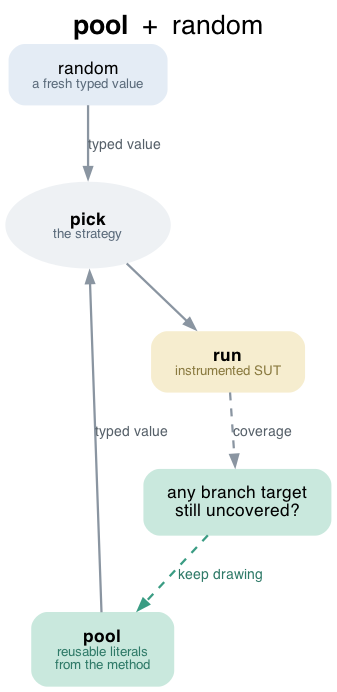
\includegraphics[width=0.40\textwidth]{../images/pool.png}\hfill
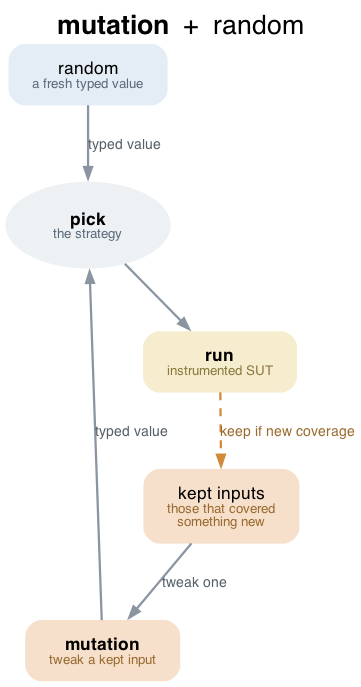
\includegraphics[width=0.40\textwidth]{../images/mutation.png}
\caption{The pool tactic (left) and the mutation tactic (right) composed with random. In every diagram, \emph{random} is one choice the strategy can pick, the chosen value is strongly typed, the instrumented SUT is run, and coverage feeds back into the tactic's state.}
\label{fig:pool}
\label{fig:mutation}
\end{figure}

\begin{figure}[t]
\centering
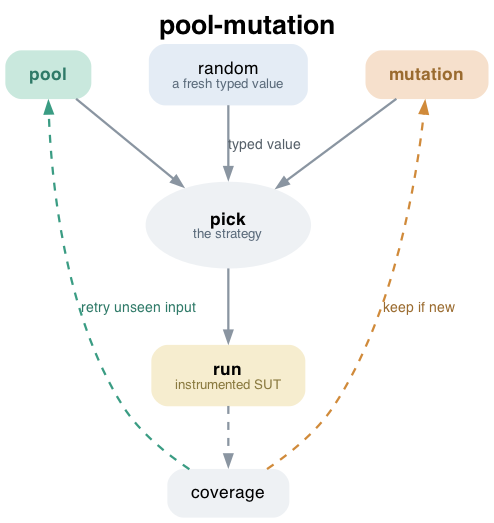
\includegraphics[width=0.46\textwidth]{../images/combined.png}
\caption{The composed strategy: pool and mutation are both available to the same strategy decision, and coverage updates the shared feedback.}
\label{fig:combined}
\end{figure}

\section{Value-Level Generation}
\label{sec:value-level}

Unlike byte-oriented fuzzers, our guidance sources operate on \emph{typed values}. A single type class describes,
for each type, how to draw a fresh value, how to mutate one, and how to draw from pooled literals. This
keeps mutations meaningful (a mutated list is still a list). The design is open: a new input type plugs in by providing one instance, and a new
strategy by deciding how to combine the available generators — nothing else changes.

% ====================================================================
\chapter{Implementation}
\label{ch:impl}

The framework is written in Scala~2.13 and split into two sbt modules: an instrumented module containing
the benchmark methods, and a dependency-light engine that hosts the framework and the experiment harness.
This chapter describes the test loop, how coverage is collected and matched to source, how method-local literals are
mined from the method body, and how each tactic is realised.

\section{Realising the Loop on ScalaCheck}
\label{sec:loop}

Pseudocode~\ref{lst:ours} is realised directly on top of ScalaCheck, so that the random strategy is the
unmodified host loop. The feedback-driven generator is built with a deferred generator that re-reads the
current feedback on every draw; the selected strategy uses a weighted choice between plain random generation
and whichever guided generators are available. The property is checked with shrinking disabled. In the
benchmark harness its body always succeeds: it exercises the SUT only to provoke coverage, snapshots that
coverage, and records it into the feedback. With the random strategy, the next generator is exactly the plain
arbitrary generator — the honest baseline. Because \texttt{scoverage}'s recording back end is process-global, each (strategy, seed) pair is
executed in its own forked JVM, and a Makefile sweeps the pairs.

\section{Binding Runtime Coverage to the Source}
\label{sec:cov-impl}

This section describes the coverage signal used by the framework.

\paragraph{Runtime view.} The benchmark module is compiled with \texttt{coverageEnabled}, so \texttt{scoverage}
instruments every statement and, at runtime, appends the identifier of each fired statement to a measurement
file. After each input the engine reads the small measurement files and maps the fired identifiers back to
scoverage's statement metadata.

\paragraph{Static view.} The statement metadata already contains the source file, method name, source span,
line number, description, and branch flag. The engine filters these statements by file and method name and
uses each remaining scoverage statement id, together with its branch flag, as one target.

\paragraph{The join.} A target is covered when its scoverage id fires. All method-local targets contribute to
statement coverage; only targets whose scoverage statements are branch-marked contribute to
branch coverage.

\paragraph{Why this binding matters.} Existing Scala coverage tooling — \texttt{scoverage}
foremost among it — already knows which instrumented statements fired. The framework keeps scoverage as the
source of truth, filters its statements to the method under test, and stores whether each target is
branch-marked by scoverage. This gives the feedback loop a source-aware signal — not only ``how much was
covered'', but which method-local targets remain uncovered. The pool mines method-local literals from the method
body with ScalaMeta, while scoverage remains the coverage source of truth; mutation retains an
input precisely when it lights up a previously-unreached target.

\section{Numeric Targets Without a Dedicated Tactic}
\label{sec:gradient}

The current implementation deliberately does not include a numeric branch-distance tactic. NumericSearch is
kept in the benchmark as a negative-control category: it contains computed or relational numeric gates where
neither literal injection nor structural mutation should be expected to provide a strong advantage over
random generation.

\section{The Pool and Mutation Tactics}
\label{sec:pool-mut}

\paragraph{Pool.} At parse time we mine method-local literals in the method body into a constant pool;
over-approximating is cheap, since a literal that fits no target is merely a wasted draw, whereas a missed
literal silently weakens the tactic. The pool source draws these reusable literals through the generator while
branch-marked targets remain uncovered. To avoid wasting effort on the same proposal, feedback records exact
inputs already executed; duplicate pool or mutation proposals fall back to random generation.

\paragraph{Mutation.} The mutation tactic perturbs the corpus of inputs that previously grew coverage. The
single most important detail is the \emph{power schedule}: it mutates the \emph{most recent} coverage-grower —
the input on the current coverage frontier — with high probability, falling back to an older seed only
occasionally. Because a mutant that breaks the frontier covers nothing new and is therefore not retained,
the search keeps springing off the best seed. Without this bias, uniform sampling over the corpus made
mutation spin on shallow seeds and fail to climb the structured benchmarks; with it, mutation reaches them.
The per-type mutators are value-level: integers take multi-scale $\pm 2^k$ steps plus edge values; lists
mutate, drop, prepend, or sort values; trees grow a leaf into a node, recurse, reorder, or prune; and tuples
mutate exactly one component, holding the rest — the operator that lets the search freeze a hard-won coordinate
and work on another.

\section{The Benchmark and the Tooling}
\label{sec:bench-impl}

The benchmark is organised as a progression of categories, each isolating one tactic's niche
(Section~\ref{sec:bench-design}). The experiment harness runs every method for one (strategy, seed) pair,
writes a JSON report per cell, and snapshots scoverage's HTML source report. A Python script then renders the
cross-strategy statement and branch charts and statistics from the JSON reports.

% ====================================================================
\chapter{Evaluation}
\label{ch:eval}

\section{Benchmark Design}
\label{sec:bench-design}

A benchmark for this question must isolate \emph{kinds} of hard branches, so that an improvement can be
attributed to a mechanism rather than to luck. We therefore designed 27 methods across five categories as a
deliberate progression (Table~\ref{tab:categories}). \emph{Calibration} methods are shallow and calibrate the
floor. \emph{MagicLiterals} methods are gated by exact literals in scalars, options, lists, tuples, or
trees — the pool's territory. \emph{MutationTargets} methods require ordered lists or shaped trees built up
incrementally — mutation's territory. \emph{MixedTargets} methods contain arms suited to both tactics, so the
composition should cover the most. \emph{NumericSearch} gates on computed or relational numeric targets that
neither literal injection nor structural mutation is expected to solve reliably.

\begin{table}[t]
\centering\small
\caption{Benchmark categories and their intended owner.}
\label{tab:categories}
\begin{tabular}{lll}
\toprule
Category & Hard-branch kind & Intended owner \\
\midrule
Calibration     & shallow / edge values              & random (floor) \\
MagicLiterals   & exact literals                     & pool \\
MutationTargets & ordered list / shaped tree         & mutation \\
MixedTargets    & several arms, one per tactic        & composition \\
NumericSearch   & computed / relational numeric      & none currently \\
\bottomrule
\end{tabular}
\end{table}

\section{Methodology}
\label{sec:methodology}

Each method is run for $10{,}000$ inputs per (strategy, seed), each pair in its own forked JVM, for
$K{=}30$ seeds — the conventional minimum for assessing randomised algorithms. Because both the baseline and
the strategies are randomised, ``the median is higher'' is not a claim on its own; following Arcuri and
Briand~\cite{arcuri2014} we report, for every strategy against random, the Vargha--Delaney $\hat{A}_{12}$
effect size — the probability that a run of the strategy beats a run of random — and the two-sided
Mann--Whitney $U$ $p$-value, both over the $30$ per-seed coverage percentages. We additionally report a
\emph{time-to-coverage} curve (coverage as a function of the input budget), a \emph{blind-spot fill} metric
(of the leaves random never reached, how many a strategy did), and \emph{throughput} (inputs per second), to
answer the cost side of the main question.

\section{Overall Results}
\label{sec:overall}

The analysis script reports suite-wide median coverage separately for statement coverage and branch-marked
statement coverage. It also emits Vargha--Delaney effect sizes and Mann--Whitney significance tests for each
guided strategy against random. The final thesis should insert the generated values from
\texttt{statement\_significance.csv} and \texttt{branch\_significance.csv}.

\section{Per-Niche Results (RQ1, RQ4)}
\label{sec:niches}

The per-category charts test whether each tactic helps in its intended niche: pool on MagicLiterals,
mutation on MutationTargets, the composition on MixedTargets, and no expected systematic winner on
NumericSearch. This directly answers RQ4: the largest improvements should occur where the program's hard
targets match a tactic's mechanism.

The final thesis should fill this section from the generated
\texttt{statement\_suite.svg}, \texttt{branch\_suite.svg}, and per-category
charts. These outputs report median coverage with min--max ranges across seeds
for random, pool, mutation, and pool-mutation.

\section{Efficiency and Cost (RQ5)}
\label{sec:cost}

The time-to-coverage curves are generated separately for statement coverage and branch coverage. They show
the median suite coverage reached after fixed input budgets, with all strategies measured through the same
instrumented loop. Throughput is reported as median inputs per second per strategy, with the guided strategies
normalised against random.

\section{Structural Findings}
\label{sec:findings}

Two findings are expected to matter beyond this implementation. First, tactics compose by proposing different
draws into the same generator, so the composite is strongest when different branches of a method are unlocked
by different mechanisms. Second, mutation is useful only when the retained corpus contains genuine
coverage-growing frontier inputs; otherwise it degenerates into a random perturbation of already-unhelpful
values.

\section{Threats to Validity}
\label{sec:threats}

\textbf{Construct.} We measure statement and branch-marked statement coverage, proxies for fault detection
rather than fault detection itself. \textbf{Internal.} Both baseline and strategies are randomised; we control
for this with repeated seeds and the Arcuri--Briand statistics, and the honest baseline removes the most common
confound. \textbf{External.} The categories are author-designed and therefore favourable to the mechanisms they
isolate. The study is confined to one language (Scala) and small methods; generalisation to large systems and
other languages is future work.

% ====================================================================
\chapter{Conclusions and Future Work}
\label{ch:conclusions}

\section{Conclusions}

This thesis set out to determine \emph{to what extent and at what cost} coverage-guided property-based testing
improves over purely random generation. The current prototype answers this by comparing random, pool,
mutation, and pool-mutation over a benchmark of 27 methods with repeated seeds, reporting both final coverage
and time-to-coverage. We also answer each auxiliary question. \textbf{RQ1}: random generation fails on
exact-literal, computed-numeric, and structured-input branches, and these are exactly where guidance can help
when a tactic matches the structure. \textbf{RQ2}: coverage can be collected cheaply by reading
\texttt{scoverage}'s measurement files after every input and mapped to method-local statement targets using
scoverage's own source and method metadata. \textbf{RQ3}: the same feedback supports literal injection and
value-level mutation, unified by one tactic interface. \textbf{RQ4}: each mechanism owns a distinct niche, and
the composition should win where several niches meet.
\textbf{RQ5}: the overhead is small because the cost is dominated by the shared instrumentation, so guidance
is worthwhile whenever the program contains branches random struggles to reach.

\section{Future Work}

The clearest opportunity is \emph{validity-guided generation} in the style of Zest~\cite{padhye2019zest}: many
hard programs demand a structurally valid input before their deeper branches become reachable, and a validity
signal would let mutation ratchet toward it. A second direction is to add a \emph{crossover}
operator so that a single branch requiring two tactics — for example a pooled integer and a sorted list —
becomes reachable, lifting the no-crossover limitation. A third is a richer \emph{power schedule} with per-seed energy,
which may let mutation contribute inside compositions rather than only in isolation. Finally, the construct
gap should be closed by evaluating fault detection directly (for instance via injected faults or mutation
testing) and by extending the study to larger, real-world systems and to other languages.

% ====================================================================
\begin{thebibliography}{99}

\bibitem{nist2002} National Institute of Standards and Technology, \emph{The Economic Impacts of Inadequate Infrastructure for Software Testing}, RTI Project 7007.011, 2002.
\bibitem{fink1997} G. Fink and M. Bishop, \emph{Property-Based Testing: A New Approach to Testing for Assurance}, ACM SIGSOFT Software Engineering Notes, 1997.
\bibitem{claessen2000} K. Claessen and J. Hughes, \emph{QuickCheck: A Lightweight Tool for Random Testing of Haskell Programs}, ICFP, 2000.
\bibitem{garousi} V. Garousi and M. V. M\"antyl\"a, \emph{When and What to Automate in Software Testing? A Multi-Vocal Literature Review}, Information and Software Technology, 2016.
\bibitem{hamlet} R. Hamlet, \emph{Random Testing}, Encyclopedia of Software Engineering, Wiley, 1994.
\bibitem{myers} G. J. Myers, C. Sandler, and T. Badgett, \emph{The Art of Software Testing}, 3rd ed., Wiley, 2011.
\bibitem{woodcock} J. Woodcock, P. G. Larsen, J. Bicarregui, and J. Fitzgerald, \emph{Formal Methods: Practice and Experience}, ACM Computing Surveys, 2009.
\bibitem{lampropoulos2019} L. Lampropoulos, M. Hicks, and B. C. Pierce, \emph{Coverage Guided, Property Based Testing}, OOPSLA, 2019.
\bibitem{padhye2019zest} R. Padhye, C. Lemieux, K. Sen, M. Papadakis, and Y. Le Traon, \emph{Semantic Fuzzing with Zest}, ISSTA, 2019.
\bibitem{padhye2019jqf} R. Padhye, C. Lemieux, and K. Sen, \emph{JQF: Coverage-Guided Property-Based Testing in Java}, ISSTA (tool track), 2019.
\bibitem{loscher2017} A. L\"oscher and K. Sagonas, \emph{Targeted Property-Based Testing}, ISSTA, 2017.
\bibitem{pacheco2007} C. Pacheco, S. K. Lahiri, M. D. Ernst, and T. Ball, \emph{Feedback-Directed Random Test Generation}, ICSE, 2007.
\bibitem{korel1990} B. Korel, \emph{Automated Software Test Data Generation}, IEEE TSE, 1990.
\bibitem{fraser2011} G. Fraser and A. Arcuri, \emph{EvoSuite: Automatic Test Suite Generation for Object-Oriented Software}, ESEC/FSE, 2011.
\bibitem{duregard2012} J. Dureg\aa rd, P. Jansson, and M. Wang, \emph{FEAT: Functional Enumeration of Algebraic Types}, Haskell Symposium, 2012.
\bibitem{mista2019} A. Mista and A. Russo, \emph{Generating Random Structurally Rich Algebraic Data Type Values} (DRAGEN2), AST, 2019.
\bibitem{afl} M. Zalewski, \emph{American Fuzzy Lop (AFL)}, \url{https://lcamtuf.coredump.cx/afl/}, 2014.
\bibitem{arcuri2014} A. Arcuri and L. Briand, \emph{A Hitchhiker's Guide to Statistical Tests for Assessing Randomized Algorithms in Software Engineering}, Software Testing, Verification and Reliability, 2014.

\end{thebibliography}

\end{document}
